\subsection{Hypothesis on Relation Properties}
\label{sec:hypothesis_relation_properties}

\begin{figure*}[htb]
\centering
\begin{minipage}{0.95\textwidth}
\centering
\small
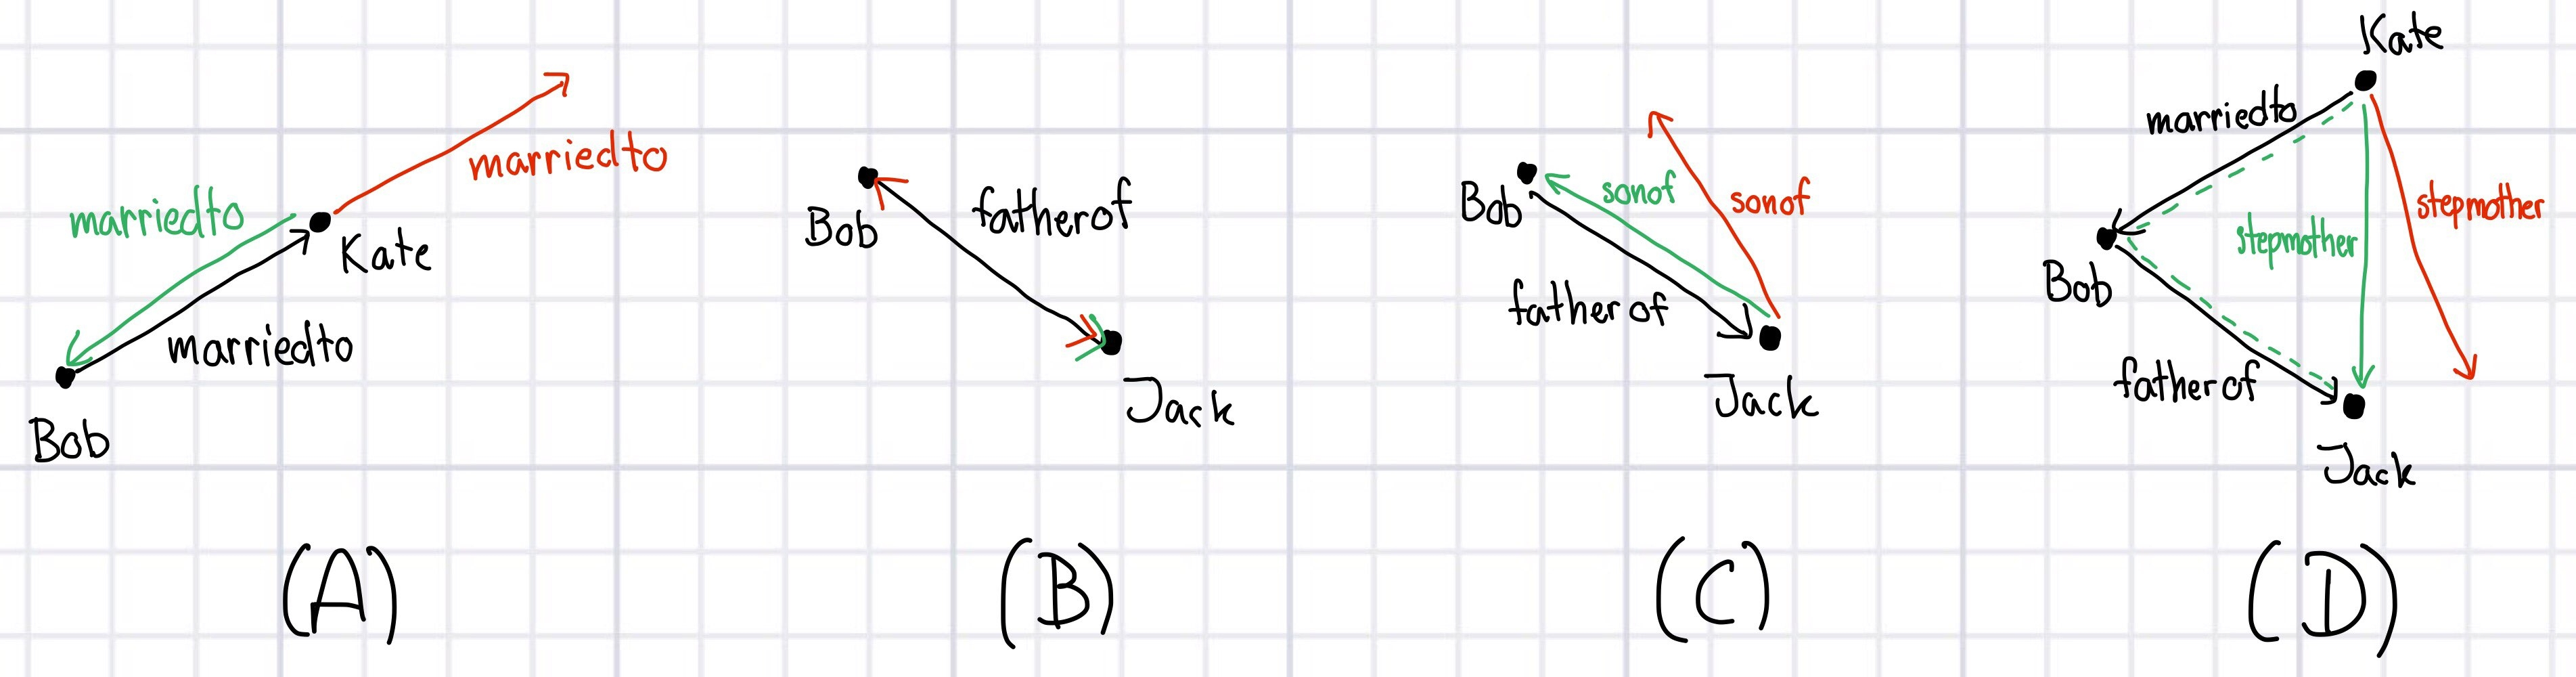
\includegraphics[scale=0.12]{content/hypotheses/figures/relation_properties_A-D.jpg}
\caption{Illustration of \autoref{hyp:relation_properties} A-D. Black is embedded information and red/green are different versions of the same relation embedding. Green is what the embedding should look like if the method can model relations with that property and red is what the embedding might look like if not. A: Symmetry, B: Anti-Symmtery, C: Inversion, D: Composition.
}
\label{fig:relation_properties_nothierarchy}
\end{minipage}
\end{figure*}

\begin{hypothesis}
\label{hyp:relation_properties}
%Prediction quality varies between models over different types of relations that are involved in the prediction task.
%Prediction quality of queries where the relation has specific properties varies between models of different embedding methods.
%Prediction quality is higher on relations with certain temporally constrained properties on methods that can express those properties, than on methods that cannot express those properties in their embeddings.
Prediction quality of queries with certain temporally constrained relation properties are better on methods which theoretically can model those properties, than methods which cannot.
\end{hypothesis}

This hypothesis is inspired by the fact that multiple embedding methods have been criticized for not handling or created in order to handle specific properties.
This hypothesis is divided into several subhypotheses specific to different models and relation properties:

\begin{subhypothesis}
\label{hyp:relation_property_sym}
DE-TransE has worse performance than other models on link prediction tasks with \textbf{symmetrical} relations.
\end{subhypothesis}

As TransE is a translational method, it is incapable of modelling symmetry \cite{goel19diachronicemb}. We suspect that DE-TransE has the same limitation with temporal symmetrical relations, which are relations that happen simultaniously between two entities. An example of such a relation could be \textit{gets\_married\_to}.

%This subhypothesis is illustrated in \autoref{fig:relation_properties_nothierarchy} A. When Bob is married to Kate, Kate is also married to Bob. If the method cannot model symmetry it may attempt to model Kate's relation to Bob with the same vector it models Bob's relation to Kate. However, in a vector space that would point Kate's relation vector in the opposite direction.

\begin{subhypothesis}
\label{hyp:relation_property_antisym}
DE-DistMult has worse performance than other models on link prediction tasks with \textbf{anti-symmetrical} relations.
\end{subhypothesis}

The DistMult method cannot model direction in the relations, and as such it cannot model anti-symmetrical relations \cite{goel19diachronicemb}. We suspect that DE-DistMult has the same problem, but for temporal anti-symmetrical relations, which are relations where an entity performs an action to another entity and that other entity cannot do the same action back in the same timespan. An example of such a relation is \textit{arrest}, as this is something a police force does to citizens, but citizens cannot do to a police force.

%This hypothesis is illustrated in \autoref{fig:relation_properties_nothierarchy} B. When Bob is the father of Jack, Jack cannot be the father of Bob. If the method cannot model anti-symmetry it may not know the direction of the vector and as such it does not know who is the father of whom.

\begin{subhypothesis}
\label{hyp:relation_property_inv}
DE-DistMult has worse performance than other models on link prediction tasks with \textbf{inverse} relations.
\end{subhypothesis}

DistMult is a method that uses pairwise interactions in diagonal matrixes, and as such it cannot model inverse relations \cite{goel19diachronicemb}. We suspect that DE-DistMult has the same problem, but for temporal inverse relations, which are relation pairs where an entity relates to another entity with one of the relations in the pair entails that there is a relation from the other entity to the first entity with the other relation in the pair, both relations happening in the same timespan. An example of such a pair is the relations \textit{host\_a\_visit} and \textit{make\_a\_visit}.

%This hypothesis is illustrated in \autoref{fig:relation_properties_nothierarchy} C. When Bob is the father of Jack, Jack is the son of Bob. If the method cannot model inversion it may embed the sonof relation separately from the fatherof relation and potentially get an entirely different result.

%\begin{subhypothesis}
%Prediction quality of queries where the relation type is a \textbf{composition} of a number of another relation types is higher on methods that can express composition than on models that can not express composition.
%\end{subhypothesis}

%This hypothesis is illustrated in \autoref{fig:relation_properties_nothierarchy} D. When Kate is married to Bob and Bob is the father of Jack, then Kate is the stepmom of Jack. Like the case for inversion, if the method cannot model composition it may embed the stepmom relation independently of its composite relations and potentially get an entirely different result.

%\begin{subhypothesis}
%Prediction quality of queries where the relation type is \textbf{reflexive} is higher on methods that can express reflexivity than on models that can not express reflexivity.
%\end{subhypothesis}

%As an example of this hypothesis, \missing[create example].


% \begin{figure}[htb]
\centering
\begin{minipage}{0.95\columnwidth}
\centering
\small
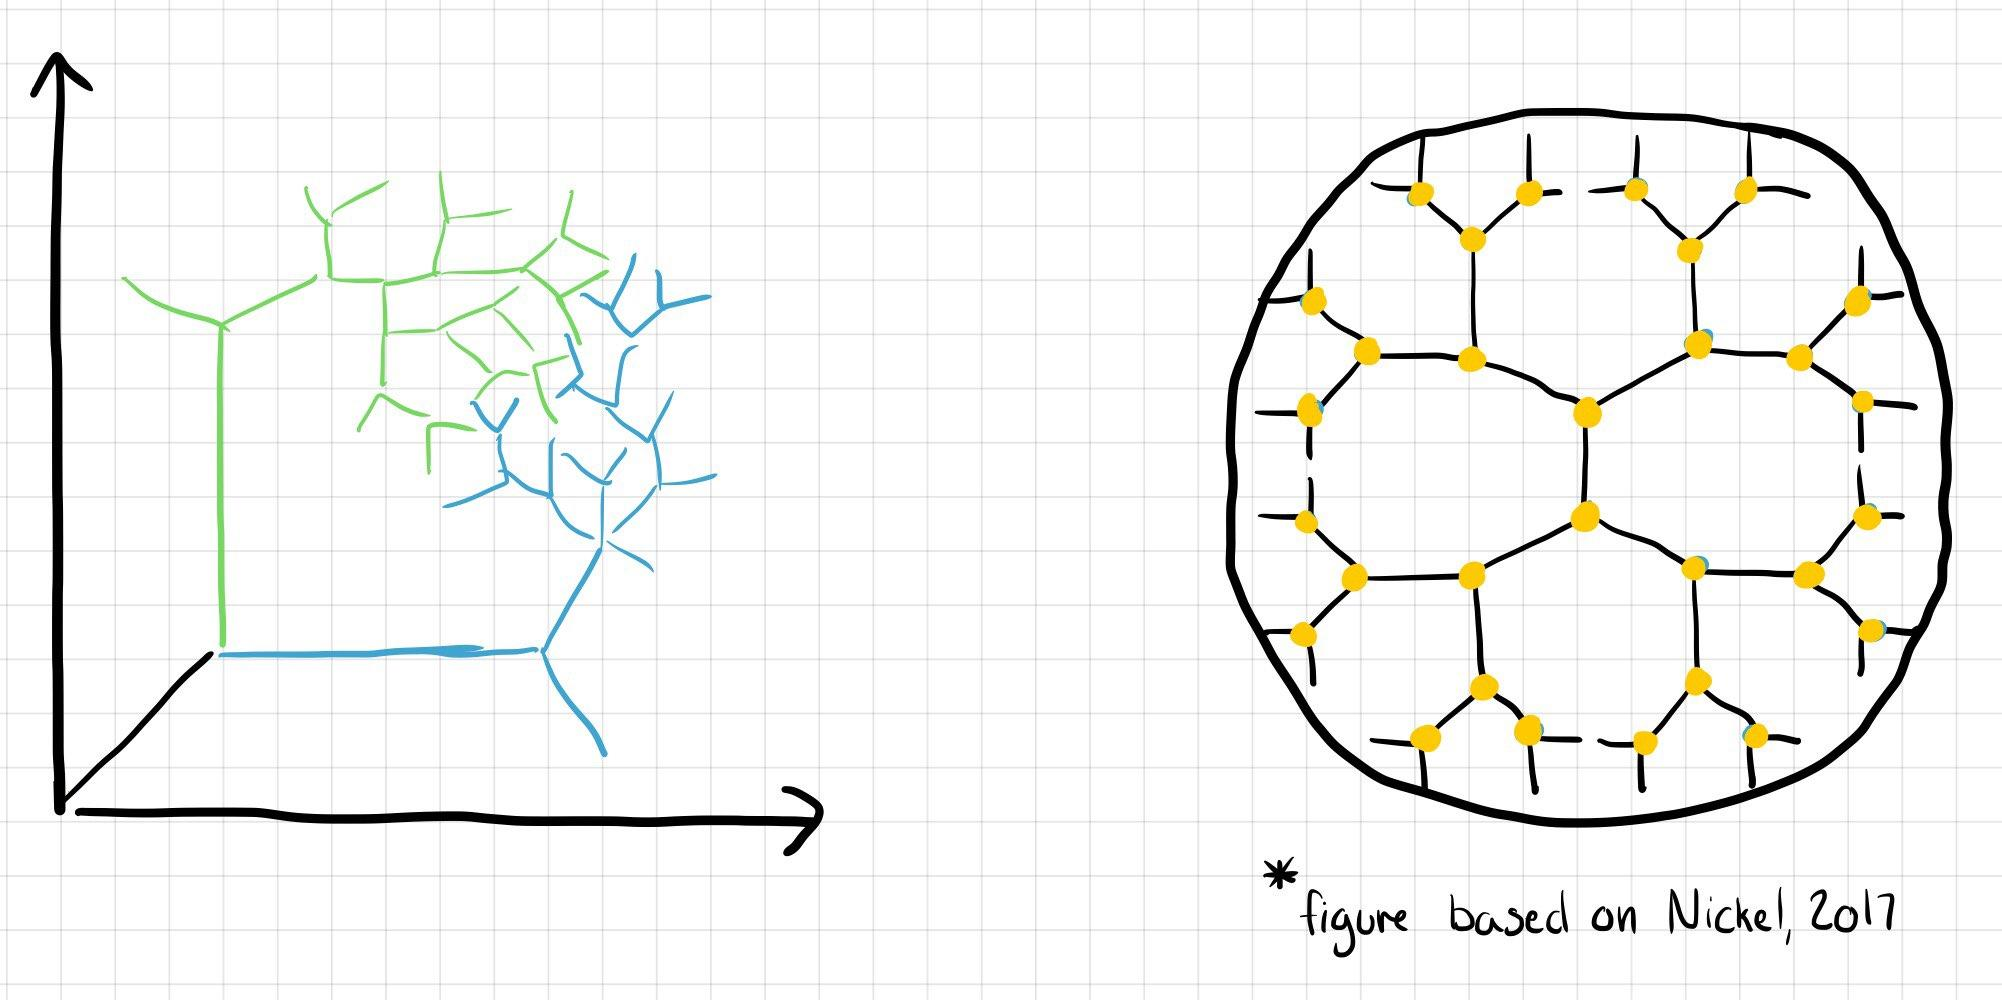
\includegraphics[scale=0.12]{content/hypotheses/figures/relation_properties_E.jpg}
\caption{Illustration of \autoref{subhyp:relation_hierarchy}. Left side shows a hierarchy embedded in Euclidian space. Right side shows a hierarchy embedded in hyperbolic space, where each yellow dot is equal distance from one another.
}
\label{fig:relation_properties_hierarchy}
\end{minipage}
\end{figure}

% \begin{subhypothesis}
% \label{subhyp:relation_hierarchy}
% Prediction quality of queries where the relation has the hierarchy property is better for models of embeddings methods within hyperbolic space.
% \end{subhypothesis}

To analyze these sub-hypotheses, and to find conclusions to the main hypothesis, a number of steps are taken to analyze the dataset and the results from the models. The first step is to assign a number of soft labels to each relation type, using a function for each relation property that maps each relation type to a real number $\varR \rightarrow [ 0 , 1 ]$. This function describes how many relations fulfill the requirements for that relation type. The reasoning for this is that knowledge graphs are not complete, and some relations might be missing from the graph.

The symmetry soft label for relation $r$ is

\begin{equation}
\begin{gathered}
\mathit{sym}(r) = \frac{|S|}{|\eta_r|}\\
S = \{ (e_1, r, e_2, \tau) \in \eta_r \mid (e_2, r, e_1, \tau) \in \eta_r \}
\end{gathered}
\end{equation}

\noindent
The anti-symmetry soft label for relation $r$ is

\begin{equation}
\begin{gathered}
\mathit{asym}(r) = \frac{|A|}{|\eta_r|}\\
A = \{ (e_1, r, e_2, \tau) \in \eta_r \mid (e_2, r, e_1, \tau) \notin \eta_r \}
\end{gathered}
\end{equation}

\noindent
The inversion soft label for relation $r$ is

\begin{equation}
\begin{gathered}
\mathit{inv}(r) = \varmax_{r^i \in \varR \setminus \{r\} } \frac{|I_{r^i}|}{|\eta_{r^i}|}\\
I_{r^i} = \{ (e_2, r^i, e_1, \tau) \in \eta_{r^i}  \mid (e_1, r, e_2, \tau) \in \eta_r \}
\end{gathered}
\end{equation}

\noindent
The reflexivity soft label for relation $r$ is

\begin{equation}
\begin{gathered}
\mathit{ref}(r) = \frac{|R|}{|\eta_r|}\\
R = \{ (e_1, r, e_2, \tau) \in \eta_r \mid e_1 = e_2 \}
\end{gathered}
\end{equation}

We then define a threshold for each of these relation traits, and classify each relation type as being symmetrical, anti-symmetrical, inverse, and/or reflexive, if the soft label for that relation type is higher than or equal to the threshold. Any relation type can have any number of these classifications. The threshold for symmetry is $0.8$, for anti-symmetry is $1.0$, for inverse is $0.8$, and for reflexivity is $0.8$. The set of facts where the relation is symmetrical ($T_S$), as well as the set of test facts where the relation is not symmetrical ($T_S'$), on testset $T$ is defined

\begin{equation}
\begin{aligned}
T_S & = \{ (h, r, t, \tau) \in T \mid \mathit{sym}(r) \geq 0.8 \}\\
T_S' & = \{ (h, r, t, \tau) \in T \mid \mathit{sym}(r) < 0.8 \}
\end{aligned}
\end{equation}

\noindent
Similarly, the anti-symmetric test facts $T_A$, the not anti-symmetric test facts $T_A'$, the inverse test facts $T_I$, the non-inverse test facts $T_I'$, the reflexive test facts $T_R$, and the non-reflexive test facts $T_R'$ are defined, using their respective thresholds.

These different test sets are then evaluated against eachother for each model, and for each dataset. If the methods that can express these relation traits have somewhat similar scores across the test sets where each individual trait is represented as the test sets where the trait is not represented, while the models that cannot represent these traits have a lower score on the test sets where they are represented compared to where they are not, the hypothesis is deemed true.

\begin{comment}
The average score for each model is then calculated for all relations that align to each of these labels, and used to calculate the most probable ranking of predictions over those relation types. The average rank of symmetrical relations on model $m$ is

%\begin{equation}
%\mathit{avg\_sym}(m) = \frac{ \varsum_{r \in \varR} \left( |\eta_r| * \mathit{sym}(r) * \frac{\varsum_{q \in \eta_r} \mathit{rank}(q , m)}{|\eta_r|} \right) }{ \varsum_{r \in \varR} |\eta_r| * \mathit{sym}(r) }
%\end{equation}

\begin{equation}
\mathit{avg\_sym}(m) = 
\frac{ \varsum_{r \in \varR} \left( \mathit{sym}(r) * \varsum_{q \in \eta_r} \frac{1}{\mathit{rank}(q , m)} \right) }
{ \varsum_{r \in \varR} |\eta_r| * \mathit{sym}(r) }
\end{equation}

\noindent
Similarly, $\mathit{avg\_asym}(m)$, $\mathit{avg\_inv}(m)$ and $\mathit{avg\_ref}(m)$ is defined, replacing $\mathit{sym}(r)$ with $\mathit{asym}(r)$, $\mathit{inv}(r)$ and $\mathit{ref}(r)$ respectively.

When a query $(h, r, t, \tau)$ is passed to the ensemble model, a weight vector $v_r \in \R^{|M|}$ is calculated for each model $m_i \in M$ from the relation $r$. This vector is defined with

\begin{equation}
v_r = \varconcat_{i = 1}^{|M|} \, \left(
\begin{aligned}
&\mathit{sym}(r) * \mathit{avg\_sym}(m_i) \, + \\
&\mathit{asym}(r) * \mathit{avg\_asym}(m_i) \, + \\
&\mathit{inv}(r) * \mathit{avg\_inv}(m_i) \, + \\
&\mathit{ref}(r) * \mathit{avg\_re}f(m_i)
\end{aligned} \right)
\end{equation}

\noindent
where $\doublepipe$ denotes concatenation between numbers, to create a vector.
\end{comment}


